%think about combining 1 and 2

% \begin{figure}[t]
%   \centering
%     %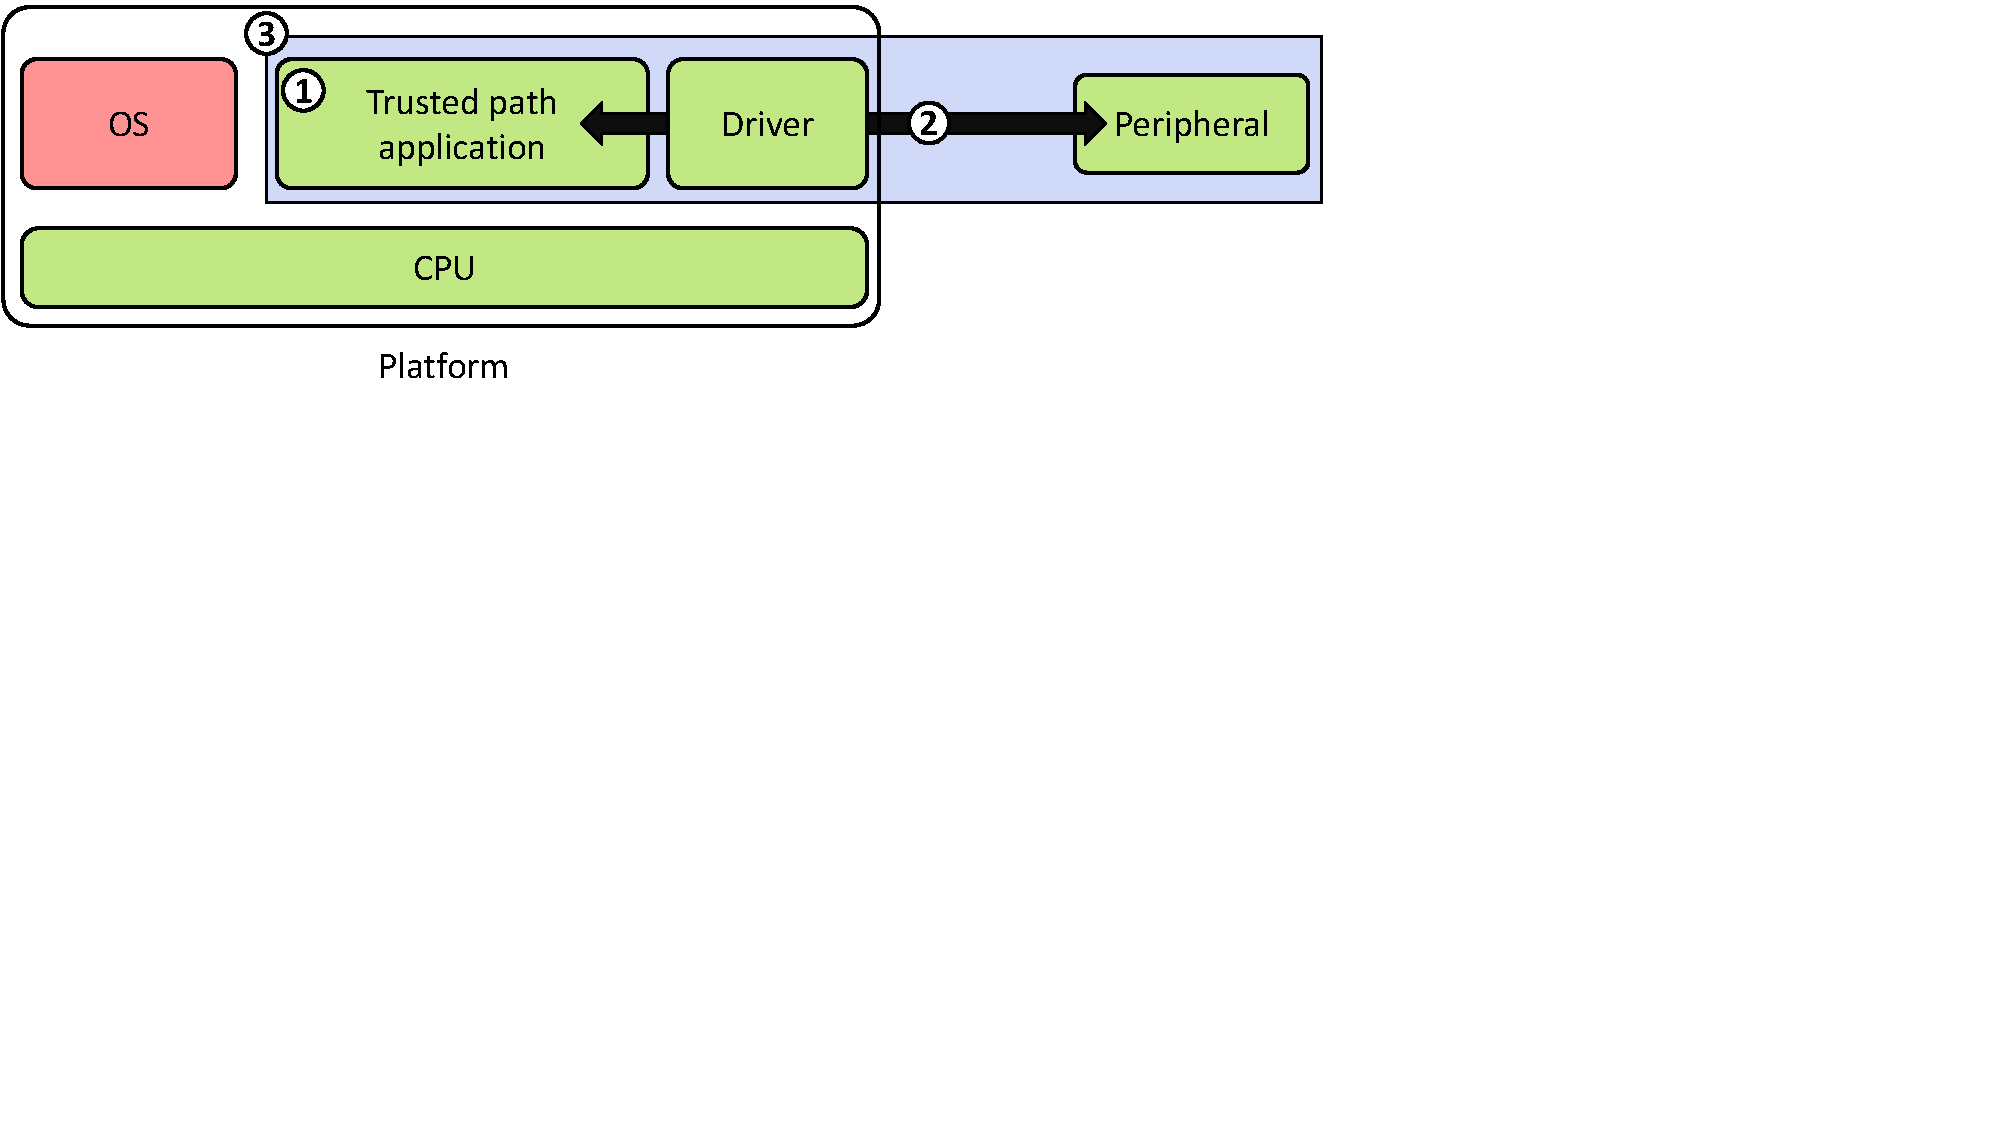
\includegraphics[trim={0 12cm 11cm 0},clip,width=\linewidth]{chapters/introduction/images/works.pdf}
%     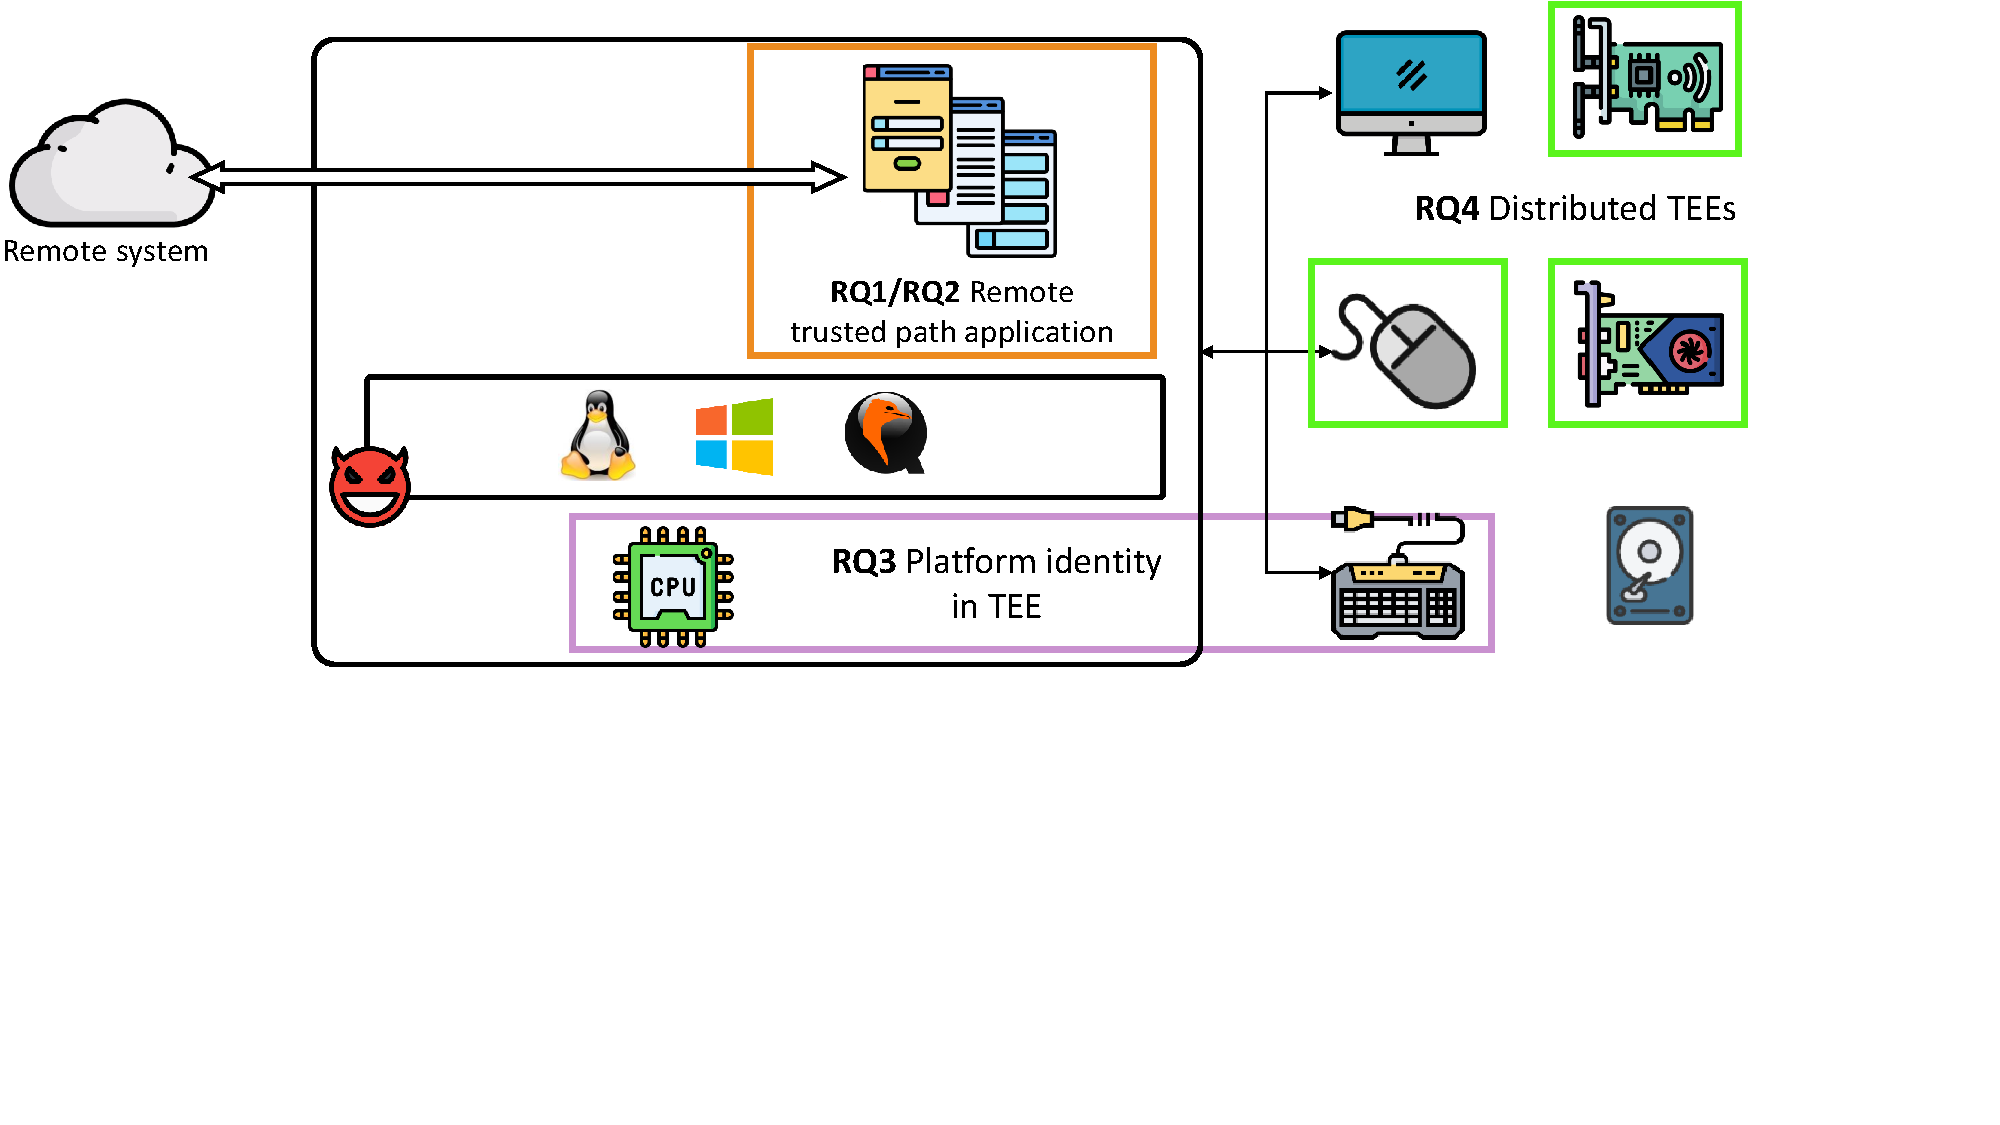
\includegraphics[trim={0 4cm 4cm 0},clip,width=\linewidth]{chapters/introduction/images/RQ.pdf}
%     \caption[Research questions]{\textbf{Research question.} In this figure, we summarize the research question that we address in this thesis a context of a modern computing platform.}
%     \label{fig:rq}
% \end{figure}

\section{Addressing the Research Question: Contribution of this Thesis}

Given the problem space discussed above, this thesis addresses the a number of research questions (RQ) concerning the trusted path and trusted execution in modern platforms.

\newtcolorbox{mybox}[2][]{colback=white!5!black,
colframe=black,fonttitle=\bfseries,
colbacktitle=black,
title=#2,#1}


\begin{mybox}[colback=white]{RQ1}
\emph{How to build trusted path systems that provide integrity (and possibly confidentiality) guarantees without the users rely on cognitive-heavy solutions such as transaction confirmation devices while maintaining a small TCB?}
\end{mybox}
  

\subsection{Addressing RQ1}
We propose two trusted path systems: \integrikey~\cite{integrikey} and \integriscreen~\cite{integriscreen} to answer \textbf{RQ1}, the first research question. \integrikey uses \emph{input signing} to provide a second factor for the integrity of the keyboard input. \integrikey leverages a small-TCB trusted embedded device to sign user input. In \integrikey, we identify a new form of input manipulation attack that we name \emph{field swapping attack} where the attacker can swap the labels of different input fields that accept overlapping values (e.g., blood pressure and heart rate for a medical implant). \integrikey analyzes the type of input fields, and based on the regular expression of these fields; it can compute the overlapping fields that could be vulnerable to swapping attack and recommend the user to append a label with the input value to distinguish it. 

In comparison, \integriscreen the uses a phone camera to extract the information that the user is typing and the UI on the screen by using text recognition to provide a second factor for user intention's integrity - that we call \emph{visual supervision}. This IO information is then sent that result to the server on a different communication channel. 

Unlike exiting trusted path solutions, these proposals rely neither on transaction confirmation devices that put a heavy cognitive load on the user nor on a hypervisor or trusted drivers that introduce a large TCB. The attacker model in \integrikey and \integriscreen differs as the latter requires trust on the smartphone for the host screen analysis. Even though both the systems provide a significant improvement over state-of-the-art trusted path solutions, they suffer similar security and functionality pitfalls as their counterparts. They are all ad-hoc approaches focus on solving a single problem and a single input source. This leads to multiple sophisticated attacks on them (e.g., character addition/reduction attack, early form submission attack, etc.). These attacks are possible not only against \integrikey or \integriscreen, but many other existing systems. The lack of security properties in these systems leads to the second research question that looks into the trusted path problem just not as a system building problem but instead addressing the fundamental security properties related to user IO operations.

\begin{mybox}[colback=white]{RQ2}
\emph{Why all\footnote{to the best of our knowledge} the existing solutions failed to provide a trusted path that provides integrity and confidentiality guarantees to the user interactions? What are the fundamental security properties required for a secure trusted path in the presence of an attacker-controlled (both software and hardware) host?}
\end{mybox}

 
    
    \subsection{Addressing RQ2}
The shortcomings of the existing literature provide the groundwork of our system named \protection that answers the first research question \textbf{RQ2}. Here we assume that the entire host (both software stack and the hardware) is attacker-controlled. We also do not assume that host has a TEE-enabled processor. \protection is built on the following observations: i) input integrity is possible only when both input and output integrity are ensured simultaneously, ii) all the input modalities are needed to be protected as they influence each other, and iii) high cognitive load results in user habituation errors. \protection uses a trusted low-TCB auxiliary device that we call \deviceprotection, which works as a mediator between all user IO devices and the untrusted host. Instead of implementing a separate network interface, the \deviceprotection uses the host as an untrusted transport - reducing the attack surface. \protection ensures output integrity and confidentiality by sending an encoded UI to the host that only the \deviceprotection can overlay on the part of the screen. The overlay is possible as the \deviceprotection intercepts the display signal between the host and the monitor. The overlay generated by the \deviceprotection ensures that the host cannot manipulate any output information on that overlaid part of the screen; hence, it can not trick the user. All the user interaction to this protected overlay is encrypted and signed by the \deviceprotection. Therefore input integrity and confidentiality are preserved.

\newpage

\begin{mybox}[colback=white]{RQ3}
\emph{Relay attack from a local platform to a remote attacker-controlled platform is a real threat to the remote attestation of TEEs like Intel SGX. How to ensure that the attacker cannot relay the attestation to an attacker-controlled platform that exposes all the sensitive IO data?}
\end{mybox}

    \subsection{Addressing RQ3}

While addressing RQ2 provides the necessary mechanisms to construct a remote trusted path application, porting the same trusted path application into a trusted execution environment (TEE) such as the Intel SGX is still non-trivial due to the relay attack on the SGX's remote attestation. Parno~\cite{parno2008bootstrapping} identified distance bounding as a candidate solution to TPM relay attacks already ten years ago but concluded that it could not be realized securely as the slow TPM identification operations (signatures) make a local and relayed attestation indistinguishable. However, the implication of the relay attack was never well-studied. In this dissertation, we investigate the implication of the relay attack and show that it could have an adverse consequence. To answer the third research question, \textbf{RQ3},  We propose a new solution, called \proximitee, that prevents relay attacks by leveraging a simple embedded device that we call \deviceproximitee that is attached to the attested target platform. The \deviceproximitee executes a challenge-response protocol between itself and the platform and based on the latency of the protocol, and the \deviceproximitee determines if it is connected to the target platform physically or not. In short, \deviceproximitee leverages distance bounding protocol to estimate the physical closeness to the target platform. Our solution is best suited (but not limited to) to scenarios where i) the deployment cost of such an embedded device is minor compared to the benefit of more secure attestation, ii) trust-on-first use (ToFU) solutions are not acceptable, and iii) most importantly, in data center scenario, simply plugging in or out the \deviceproximitee allocate or revoke a specific platform from a data center fleet without explicitly relying on a public key ledger. Attestation of servers at cloud computing platforms and setup of SGX-based permissioned blockchains are two such examples. Note that, in contrast to the earlier research questions (RQ1 and RQ2), we only assume that the software stack and the network is fully attacker-controlled and the CPU to be trusted.
    
    
    \begin{mybox}[colback=white]{RQ4}
\emph{How to extend the trusted path mechanism to a modern platform that is interconnected with a number of heterogeneous peripheral devices? These peripherals can range range IO devices to other complex hardware devices such as GPU or accelerator that can execute programs outside the CPU cores. How to ensure the platform-wide integrity guarantee (configuration and interaction of the TEE enclaves and external peripherals) is preserved without relying on a purpose-built system?}
\end{mybox}
    
   

\subsection{Addressing RQ4}
Finally, to answer \textbf{RQ4}, the last research question, We propose a TEE with a \emph{configurable} software and hardware TCB including arbitrary external peripheral devices, a concept that we name \emph{platform isolation environment} (\pie). \pie executes applications in \emph{platform-wide enclaves}, which are analogous to the enclaves provided by TEEs, except that they span several hardware components. For example, a \nameenclave{} can be composed of an output device such as a display, input devices such as keyboard and mouse, the CPU that is executing the program, the GPU that renders the graphics, and the custom code running on them. Like in traditional enclaves, a \nameenclave{} can be remotely attested. However, the \pie attestation not only reports a measurement of the software TCB but also of the hardware components that are part of the \nameenclave{}.


The shift towards configurable hardware and software TCBs has wide-ranging implications concerning integrity, confidentiality, and attestation of a \nameenclave{}. 
Attestation, for one, should cover all individual components of a \nameenclave{} atomically to defend against an attacker that changes the configuration in between attestations to separate components. 
Moreover, the untrusted OS may remap the peripheral devices at runtime with an untrustworthy device, which should not receive access to sensitive data. We carefully design \pie to not be vulnerable to such attacks and present an in-depth security analysis.

We mitigate the above-mentioned attacks with two new properties of \nameenclave{}s: \emph{platform-wide attestation} and \emph{platform awareness}. Platform-wide attestation expands the attestation to cover all components within a \nameenclave, and platform awareness enables enclaves to react to changes in their ecosystem, i.e., remapping by the OS.
We achieve this by introducing two new events into the enclave lifecycle, \textit{connect} and \textit{disconnect}, which allow to track the liveliness of one enclave from another.


A summary of all above-mentioned research questions are depicted in Figure~\ref{fig:works}. Additionally, the figure provides an overview of all the works in this thesis that address these research question.

\begin{figure}[t]
  \centering
    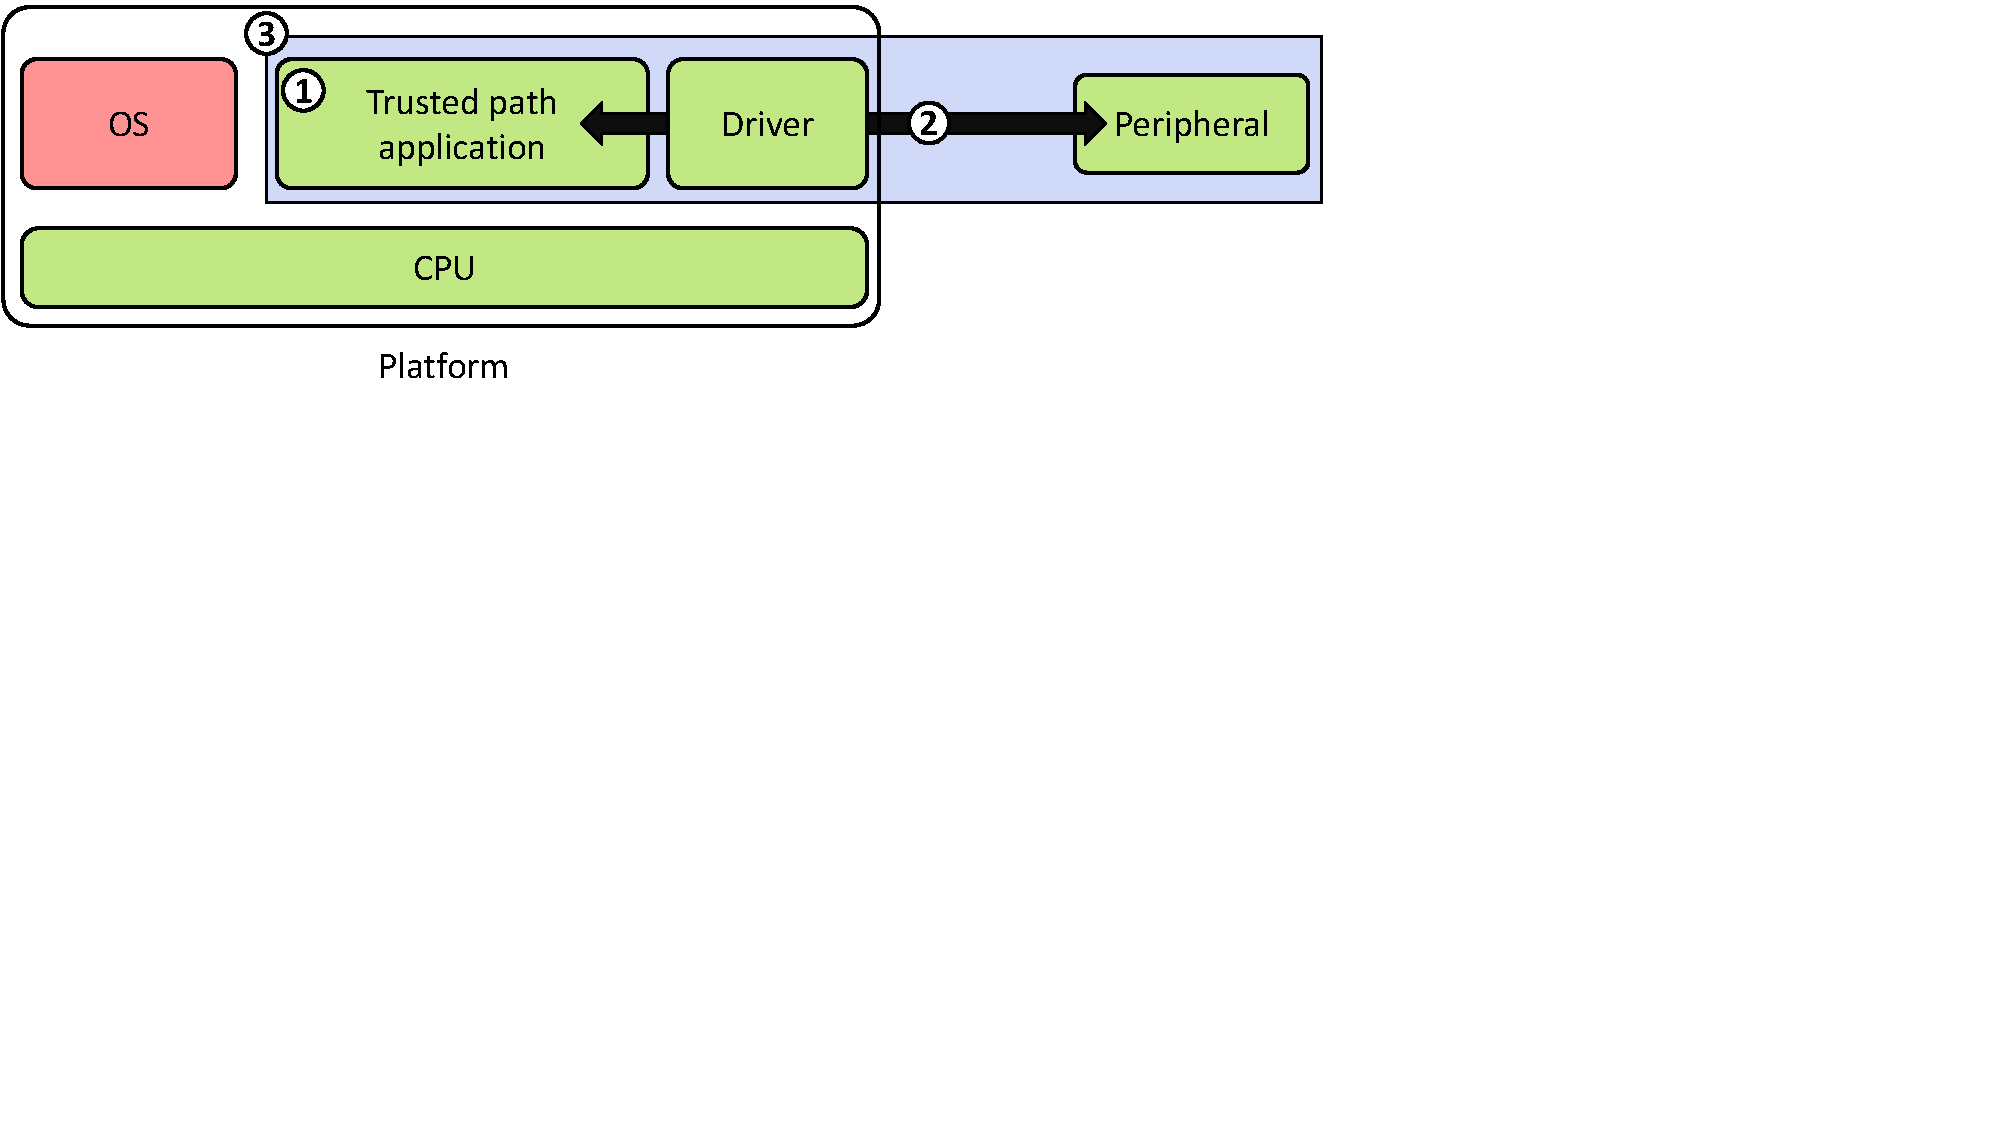
\includegraphics[trim={0 3cm 4cm 0},clip,width=\linewidth]{chapters/introduction/images/works.pdf}
    \caption[Summary of the works in this thesis]{\textbf{Summary of the works in this thesis.} In this figure, we summarize the works that are in the thesis in a context of a modern computing platform.}
    \label{fig:works}
\end{figure}